
\section{Muhammad Afra Faris/1174041}
\subsection{Soal 1}
Fungsi, Sejarah, dan Contoh file CSV : 
\begin{itemize}
	\item Fungsi : 
	File Comma Separated Values atau  biasa disingkat dengan CSV merupakan tipe file khusus yang menyimpan informasi dengan metode dipisahkan dengan koma. File CSV berfungsi untuk menjadi perantara beberapa aplikasi yang memiliki basis data saat pengiriman data. CSV juga dapat dibuka di berbagai text editor. Dengan bentuk filenya yang dinamis, file CSV mungkin dapat dimanipulasi dan dapat menyimpan informasi dengan skala besar.
	\item Sejarah :
	CSV ini sudah digunakan sejak tahun 1972 yang dapat dikompilasi pada bahasa pemrograman IBM Fortran. Pada saat itu, data yang dipisahkan oleh koma jika isinya memiliki spasi maka harus diberi tanda petik di awal dan akhir isi dari data tersebut. Nama CSV ini baru mulai digunakan pada tahun 1983. Pada panduan dari Osborne Executive Computer mendokumentasikan kutipan yang membolehkan isi karakter memiliki koma.  Tahun 2005 dengan RFC4180, CSV didefinisikan sebagai MIME Content Type. lalu pada tahun 2013, defisiensi dari RFC4180 dipecahkan oleh rekomendasi dari W3C. Tahun 2014, IETF mempublikasi RFC7111 yang mendeskripsikan pecahan Uniform Resource Identifier(URI) ke dokumen CSV. RFC7111 menjelaskan bagaimana baris, kolom dapat dipilih dalam dokumen CSV menggunakan indeks posisi. Pada Tahun 2015,  draft rekomendasi untuk CSV-metadata standards dipublikasikan W3C yang dimulai dengan rekomendasi pada bulan Desember dengan tahun yang sama. 
	\item Contoh File CSV \begin{itemize}
							\item 
							CSV pada Excel \ref{csvex}
							\begin{figure}[!htbp]
								\centering
								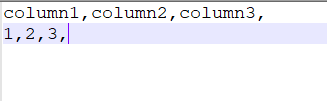
\includegraphics[height=4cm, width=7cm]{figures/4/1174041/Teori/csvex.png}
								\caption{Contoh CSV Pada Excel}
								\label{csvex}
							\end{figure}
														
						  \end{itemize}
\end{itemize}
\subsection{Soal 2}
Aplikasi Yang dapat membuat file CSV : 
Berikut file yang dapat membuat file CSV
\begin{itemize}
	\item Spreadsheet :
	Spreadsheet adalah aplikasi yang bisa digunakan membuat CSV hanya dengan memasukan data sesuai baris dan kolom yang diinginkan. Contoh dari spreadsheet seperti Microsoft Excel, Google Spreadsheet, dan beberapa aplikasi lainnya. 
	\item Bahasa Pemrograman :
	Bahasa pemrograman adalah sarana media yang dapat digunakan untuk membuat aplikasi, yang bisa membuat file CSV khusus untuk bahasa pemrograman yang mendukung dengan pembuatan file CSV. Seperti Python, C Sharp, dan lain sebagainya.
	\item Text Editor :
	Text editor juga dapat digunakan untuk membuat file CSV. Untuk membuat file CSV dengan Text Editor cukup dengan membuat file sesuai format CSV dan save file tersebut dengan ekstensi .CSV.
\end{itemize}
\subsection{Soal 3}
Menulis dan Membaca file CSV : 
Berikut cara menulis dan membaca file CSV : 
\begin{itemize}
	\item Menulis : \begin{enumerate}
						\item Buka file CSV dengan spreadsheet apapun
						\item Klik Cell yang akan dimasukkan
						\item Masukan data yang akan dimasukkan pada cell tersebut
						\item Lalu save file dengan format .CSV
					\end{enumerate}
	\item Membaca : \begin{enumerate}
						\item Buka file CSV dengan spreadsheet						
					\end{enumerate}
\end{itemize}
\subsection{Soal 4}
Sejarah Library CSV Python : 
Library CSV pada python merupakan library yang paling umum untuk import export data pada spreadsheet dan basis data dengan format sesuai dengan standarisasi RFC4180. Seiring dengan lahirnya bahasa pemrograman python, library mulai dibuat dan dikembangkan sampai akhirnya pada tahun 2003, pembuatnya Kevin Altis dan lainnya telah merilis versi final untuk library Python CSV. 
\subsection{Soal 5}
Sejarah Library Pandas Python : 
Pandas (Python Data Analysis Library) adalah library open source yang digunakan untuk melakukan data manajemen dan data analysis. Pandas diciptakan pada tahun 2008 oleh Wes McKinney dan diperbaharui oleh Sien Chang pada tahun 2010. Inspirasi dari pembuatan pandas muncul pada komunitas yang membutuhkan library khusus untuk analisis data. 
\subsection{Soal 6}
Fungsi - fungsi yang terdapat di library CSV : 
\begin{itemize}
	\item \begin{verbatim} csv.reader(csvfile, dialect='excel', **fmtparams) \end{verbatim} Untuk mengembalikan	object reader yang akan mengambil setiap line pada csv yang diambil. Data setiap baris diambil saat next() dipanggil. 
	\item \begin{verbatim} csv.writer(csvfile, dialect='excel', **fmtparams) \end{verbatim} Mengembalikan file pembuat object untuk dapat mengkonversi data pada python ke file CSV yang akan dibuat. 
	\item \begin{verbatim} csv.register_dialect(name[, dialect[, **fmtparams]]) \end{verbatim} Mengasosiasikan dialek dengan nama, dan nama yang dimasukkan harus berupa karakter.
	\item \begin{verbatim} csv.unregister_dialect(name) \end{verbatim}
	Menghapus asosiasi dialek dengan nama yang ada pada registry dialek.
	\item \begin{verbatim} csv.get_dialect(name) \end{verbatim}
	Mengambil dialek yang telah diasosiasikan dengan nama. 
	\item \begin{verbatim}  csv.list_dialects() \end{verbatim} Mengembalikan dialek yang telah terregistrasi.
	\item \begin{verbatim} csv.field_size_limit([new_limit]) \end{verbatim} Mengembalikan maksimal column data yang diperbolehkan oleh pembaca.
\end{itemize}
\subsection{Soal 7}
Fungsi - fungsi yang terdapat di library Pandas : 
\begin{itemize}
	\item \begin{verbatim} pandas.read_excel(io[, sheet_name, header, names, …])  \end{verbatim} Membaca file excel dan menyimpan ke DataFrame.
	\item \begin{verbatim} pandas.read_csv(filepath_or_buffer[, sep, …]) \end{verbatim} Untuk membaca file CSV dan menyimpan ke DataFrame.
	\item \begin{verbatim} to_csv([path, index, sep, na_rep, …]) \end{verbatim}
	Untuk membuat file CSV dari data yang telah ada.	
\end{itemize}
\subsection{Cek Plagiarism}
Berikut pengecekan plagiarism yang dilakukan pada website smallseotools.com : 
\begin{figure}[!htbp]
	\centering
	
\includegraphics[height=6cm, width=10cm]{figures/4/1174041/Teori/plagiarism.png}
	\caption{Cek Plagiarisme}
	\label{plagiarism}
\end{figure}

\section{Rangga Putra Ramdani}
\subsection{Fungsi Csv}
Fungsi csv yaitu memudahkan user dalam melakukan input data karena pada csv input data ataupun import data dalam skala besar dapat dilakukan dengan cara yang sederhana.
\subsection{Sejarah Csv}
Dari rilis pertama, Excel menggunakan format file biner yang disebut Binary Interchange File Format (BIFF) sebagai format file utamanya. Ini berubah ketika Microsoft merilis Office System 2007 yang memperkenalkan Office Open XML sebagai format file utamanya. Office Open XML adalah file kontainer berbasis XML yang mirip dengan XML Spreadsheets (XMLSS), yang diperkenalkan di Excel 2002. File versi XML tidak bisa menyimpan makro VBA. Meskipun mendukung format XML baru, Excel 2007 masih mendukung format lama yang masih berbasis BIFF tradisional. Selain itu Microsoft Excel juga mendukung format Comma Separated Values (CSV), DBase File (DBF), SYMbolic LinK (SYLK), Format Interchange Data (DIF) dan banyak format lainnya, termasuk format lembar kerja 1-2 Lotus - 3 (WKS, WK1, WK2, dll.) Dan Quattro Pro.
\lstinputlisting[firstline=7, lastline=20]{src/4/1174056/teori/Shasa.py}
\subsection{Aplikasi yang dapat menghasilkan csv}
\begin{itemize}
\item Texteditor
Seperti notepad++,visual studio code,atom,sublime dan lain sebagainya
\item Program Spreadsheet
  Seperti excell,google spreadshare,LibreOfficecalc
 \end{itemize}
\subsection{Jelaskan bagaimana cara menulis dan membaca file csv di excel atau spreadsheet}
Caranya sangat mudah yaitu:
 Untuk menulisnya untuk yang paling atas itu kita buat headernya,untuk mepermudah membedakan datanya,dan untuk baris kedua dan seterusnya itu untuk data itu sendiri.Setelah di buat kalian save as kemudian pilih format CSV.Untuk membukan cukup di double clik file tersebut
\subsection{Jelaskan sejarah library csv}
CSV muncul untuk memudahkan data science dan analis karena dinilai terdapat banyak kemudahan yang didapat. CSV dapat dimaksimalkan jika dipaduka dengan python karena python adalah bahasa pemrograman yang support ke banyak library termasuk csv. Maka karena itulah perpaduan python dan csv seringkali digunakan oleh perusahaan-perushaan besar dalam mengolah datanya.
\subsection{Jelaskan sejarah library pandas}
Pandas merupakan tool yang dapat digunakan sebagai alat analisis data dan struktur untuk bahasa pemrograman Python. Pandas dapat mengolah data dengan mudah, salah satu fitur yang ada dalam pandas adalah Dataframe. Fitur dataframe dapat membaca sebuah file dan menjadikannya tabble, juga dapat mengolah suatu data dengan menggunakan operasi seperti join, group by dan teknik lainnya yang terdapat pada SQL. Dalam hal ini pandas tidak jauh beda dengan csv yaitu memiliki keunggulan dalam pengolahan data-data besar dan dapat disupport dengan baik dengan python walaupun mengimport data dalam jumlah banyak.
\subsection{Fungsi-fungsi Library CSV}
Dalam library csv terdapat dua fungsi yaiut fungsi membaca file dan menulis file csv.
Library csv mempunyai keunggulan dibandingkan format data lainnya adalah soal kompatibilitas. File csv dapat digunakan, diolah, diekspor/impor, dan dimodifikasi menggunakan berbagai macam perangkat lunak dan bahasa pemrograman. Pada library csv mempunyai fungsi import dan eksport data yang baik dan bisa digunakan dalam jumlah besar.
\subsection{Fungsi-fungsi library Pandas}
Pandas pun memiliki fungsi yang sama yaitu menulis dan membaca file. pandas menyediakan beragam fungsi operasi untuk mengolah data. Contoh jika menggunakan series bisa mencari nilai max, min, dan mean secara langsung, bahkan juga bisa melakukan operasi perpangkatan pada nilai Series secara langsung.
Pandas dapat mengolah suatu data dan mengolahnya seperti join, distinct, group by, agregasi, dan teknik seperti pada SQL. Hanya saja dilakukan pada tabel yang dimuat dari file ke RAM.

\section{Teddy Gideon Manik}
\subsection{Soal 1}
Comma Separated Value atau CSV adalah format data yang memudahkan penggunanya melakukan input data ke database secara sederhana. CSV dapat digunakan dalam standar file ASCII. Dalam format csv record dipisahkan dengan tanda koma atau titik koma. Ketika user menerima file dengan format CSV, yang biasanya bertuliskan .CSV, maka file tersebut akan terbuka dalam format Microsoft Excel. CSV muncul demi memenuhi kebutuhan perusahaan-perusahaan besar dalam mengolah data yang banyak.
\lstinputlisting[firstline=7, lastline=20]{src/4/1174038/teori/coba.py}
\subsubsection{Fungsi}
Fungsi csv yaitu memudahkan user dalam melakukan input data karena di csv input data atau import data dalam skala besar dapat dilakukan dengan cara yang sederhana.
\subsection{Soal 2}
Ada beberapa aplikasi yang dapat menghasilkan file dengan format csv diantaranya google sheet, number di MacOS dan microsoft excel.
\subsection{Soal 3}
cara membuat file csv di excel cukup mudah yaitu :
\begin{itemize}
	\item Buat foldernya
	\item Pilih save as
	\item pilih file dengan format csv
\end{itemize}
cara membaca file di csv :
\begin{itemize}
	\item Klik data get external data form text
	\item Akan muncul Text Import Wizard, arahkan pada file csv yang ingin anda buka Open.
	\item Setelah File terbuka, akan muncul Text Import Wizard.
	\item Pilih Delimited, Kemudian Next (Di sini, bisa juga menentukan baris awal yang akan di import)
	\item Centrang pada Tab dan Comma (Atau sesuai pengaturan File Anda) Next.
	\item Atur Format data pada tiap kolom yang tampil dan klik Finish
\end{itemize}
\subsection{Soal 4}
CSV muncul untuk memudahkan data science dan analis karena dinilai terdapat banyak kemudahan yang didapat. CSV dapat dimaksimalkan jika dipaduka dengan python karena python adalah bahasa pemrograman yang support ke banyak library termasuk csv. Maka karena itulah perpaduan python dan csv seringkali digunakan oleh perusahaan-perushaan besar dalam mengolah datanya.
\subsection{Soal 5}
Pandas merupakan tool yang dapat digunakan sebagai alat analisis data dan struktur untuk bahasa pemrograman Python. Pandas dapat mengolah data dengan mudah, salah satu fitur yang ada dalam pandas adalah Dataframe. Fitur dataframe dapat membaca sebuah file dan menjadikannya tabble, juga dapat mengolah suatu data dengan menggunakan operasi seperti join, group by dan teknik lainnya yang terdapat pada SQL. Dalam hal ini pandas tidak jauh beda dengan csv yaitu memiliki keunggulan dalam pengolahan data-data besar dan dapat disupport dengan baik dengan python walaupun mengimport data dalam jumlah banyak.
\subsection{Soal 6}
Dalam library csv terdapat dua fungsi yaiut fungsi membaca file dan menulis file csv.
Library csv mempunyai keunggulan dibandingkan format data lainnya adalah soal kompatibilitas. File csv dapat digunakan, diolah, diekspor/impor, dan dimodifikasi menggunakan berbagai macam perangkat lunak dan bahasa pemrograman. Pada library csv mempunyai fungsi import dan eksport data yang baik dan bisa digunakan dalam jumlah besar.
\subsection{Soal 7}
Pandas pun memiliki fungsi yang sama yaitu menulis dan membaca file. pandas menyediakan beragam fungsi operasi untuk mengolah data. Contoh jika menggunakan series bisa mencari nilai max, min, dan mean secara langsung, bahkan juga bisa melakukan operasi perpangkatan pada nilai Series secara langsung.
Pandas dapat mengolah suatu data dan mengolahnya seperti join, distinct, group by, agregasi, dan teknik seperti pada SQL. Hanya saja dilakukan pada tabel yang dimuat dari file ke RAM.

\section{Harun Ar-Rasyid}
\subsection{Soal 1}
Isi jawaban soal ke-1

Kalau mau dibikin paragrap \textbf{cukup enter aja}, tidak usah pakai \verb|par| dsb

%\subsection{Soal 2}
%Isi jawaban soal ke-2

%\subsection{Soal 3}
%Isi jawaban soal ke-3

\section{Sri Rahayu}
\subsection{Soal 1}
Isi jawaban soal ke-1

Kalau mau dibikin paragrap \textbf{cukup enter aja}, tidak usah pakai \verb|par| dsb

%\subsection{Soal 2}
%Isi jawaban soal ke-2

%\subsection{Soal 3}
%Isi jawaban soal ke-3

\section{Doli Jonviter}
\subsection{Soal 1}
Isi jawaban soal ke-1

Kalau mau dibikin paragrap \textbf{cukup enter aja}, tidak usah pakai \verb|par| dsb

%\subsection{Soal 2}
%Isi jawaban soal ke-2

%\subsection{Soal 3}
%Isi jawaban soal ke-3

\section{Rahmatul Ridha}
\subsection{Soal 1}
Isi jawaban soal ke-1

Kalau mau dibikin paragrap \textbf{cukup enter aja}, tidak usah pakai \verb|par| dsb

%\subsection{Soal 2}
%Isi jawaban soal ke-2

%\subsection{Soal 3}
%Isi jawaban soal ke-3

\section{Tomy Prawoto}
\subsection{Soal 1}
Isi jawaban soal ke-1

Kalau mau dibikin paragrap \textbf{cukup enter aja}, tidak usah pakai \verb|par| dsb

%\subsection{Soal 2}
%Isi jawaban soal ke-2

%\subsection{Soal 3}
%Isi jawaban soal ke-3

